\chapter{Background}
\label{ch:background}
This chapter will present the necessary background information for this thesis. Here, we define some basic terminology that will be used throughout this thesis.

\section{Code clone terminology}\label{sec:terminology}
Many studies present different definitions for code clone concepts. For this study, we mainly use the definitions from Bruntink et al. \cite{bruntink2005use}, Roy et al. \cite{roy2007survey} and Jiang et al. \cite{jiang2007deckard}. We created a summary of these concepts, which can be found in table \ref{tab:clone-terminology}.

\begin{table}[H]
\centering
\resizebox{\textwidth}{!}{%
\begin{tabular}{@{}llll@{}}
\toprule
\rowcolor[HTML]{FFFFFF}
\textbf{Symbol} & \textbf{Meaning} & \textbf{Description} & \textbf{Properties} \\ \midrule
\rowcolor[HTML]{EFEFEF}
S & \begin{tabular}[c]{@{}l@{}}Clone class\\ collection\end{tabular} & \begin{tabular}[c]{@{}l@{}}All clone classes that have been\\found for a certain software\\project.\end{tabular} & \textbf{Clones:} Set of clone classes. \\
\rowcolor[HTML]{FFFFFF}
C & Clone class & \begin{tabular}[c]{@{}l@{}}A set of similar code fragments in\\ different locations.\end{tabular} & \textbf{Instances:} Set of clone instances. \\
\rowcolor[HTML]{EFEFEF}
I & \begin{tabular}[c]{@{}l@{}}Clone\\ instance\end{tabular} & \begin{tabular}[c]{@{}l@{}}A code fragment that appears in\\ multiple locations.\end{tabular} & \begin{tabular}[c]{@{}l@{}}\textbf{Contents:} Totally ordered set of nodes, ordered\\by their begin positions.\\ \textbf{File:} The file in which this clone instance is \\ found.\\ \textbf{Range:} The range this clone instance spans.\end{tabular} \\
\rowcolor[HTML]{FFFFFF}
N & Node & \begin{tabular}[c]{@{}l@{}}A statement or declaration in a \\ codebase.\end{tabular} & \textbf{Range:} The range this node spans. \\
\rowcolor[HTML]{EFEFEF}
R & Range & A part of a source code file. & \begin{tabular}[c]{@{}l@{}}\textbf{Tokens:} Set of tokens that this range spans.\\ \textbf{Begin line/column:} The line and column at \\ which the range starts.\\ \textbf{End line/column:} The line and column at\\ which the range end.\end{tabular} \\
\rowcolor[HTML]{FFFFFF}
T & Token & \begin{tabular}[c]{@{}l@{}}Tokens are the basic lexical\\ building blocks of source code. \\ For this study, this is the smallest\\ relevant entity of a program.\end{tabular} & \begin{tabular}[c]{@{}l@{}}\textbf{Range:} The range this token spans.\\ \textbf{Category:} Identifier, Keyword, Literal, Separator, \\ Operator, Comment or Whitespace\end{tabular} \\ \bottomrule
\end{tabular}%
}
\caption{Clone related terminology and how it maps to the source code.}
\label{tab:clone-terminology}
\end{table}

\subsection{Example}
The code fragment in figure \ref{fig:cloneclasses} shows two clone classes. One of the clone classes consists of two clone instances and has three nodes per instance. The other clone instance has three clone instances and consists of two nodes per instance.

\definecolor{lightyellow}{HTML}{fffdcc}
\newcommand{\highlightYellow}{\makebox[0pt][l]{\color{lightyellow}\rule[-4pt]{1\linewidth}{14pt}}}
\newcommand{\highlightDarkyellow}{\makebox[0pt][l]{\color{yellow}\rule[-4pt]{1\linewidth}{14pt}}}
\begin{figure}[H]
\begin{parcolumns}{3}
\colchunk[1]{
\begin{javacode}
// File1.java
|\highlightDarkyellow|doA();
|\highlightDarkyellow|doB();
|\highlightYellow|doC();
\end{javacode}}
\colchunk[2]{
\begin{javacode}
// File2.java
|\highlightDarkyellow|doA();
|\highlightDarkyellow|doB();
|\highlightYellow|doC();
\end{javacode}}
\colchunk[3]{
\begin{javacode}
// File3.java
|\highlightYellow|doA();
|\highlightYellow|doB();
doD();
\end{javacode}}
\end{parcolumns}
\caption{Two clone classes: One clone class with three clone instances and one with two clone instances.}
\label{fig:cloneclasses}
\end{figure}

This example can be represented as a tree structure using the concepts from table \ref{tab:clone-terminology}. This tree structure is displayed in figure \ref{fig:terminologyexample}.

\begin{figure}[H]
  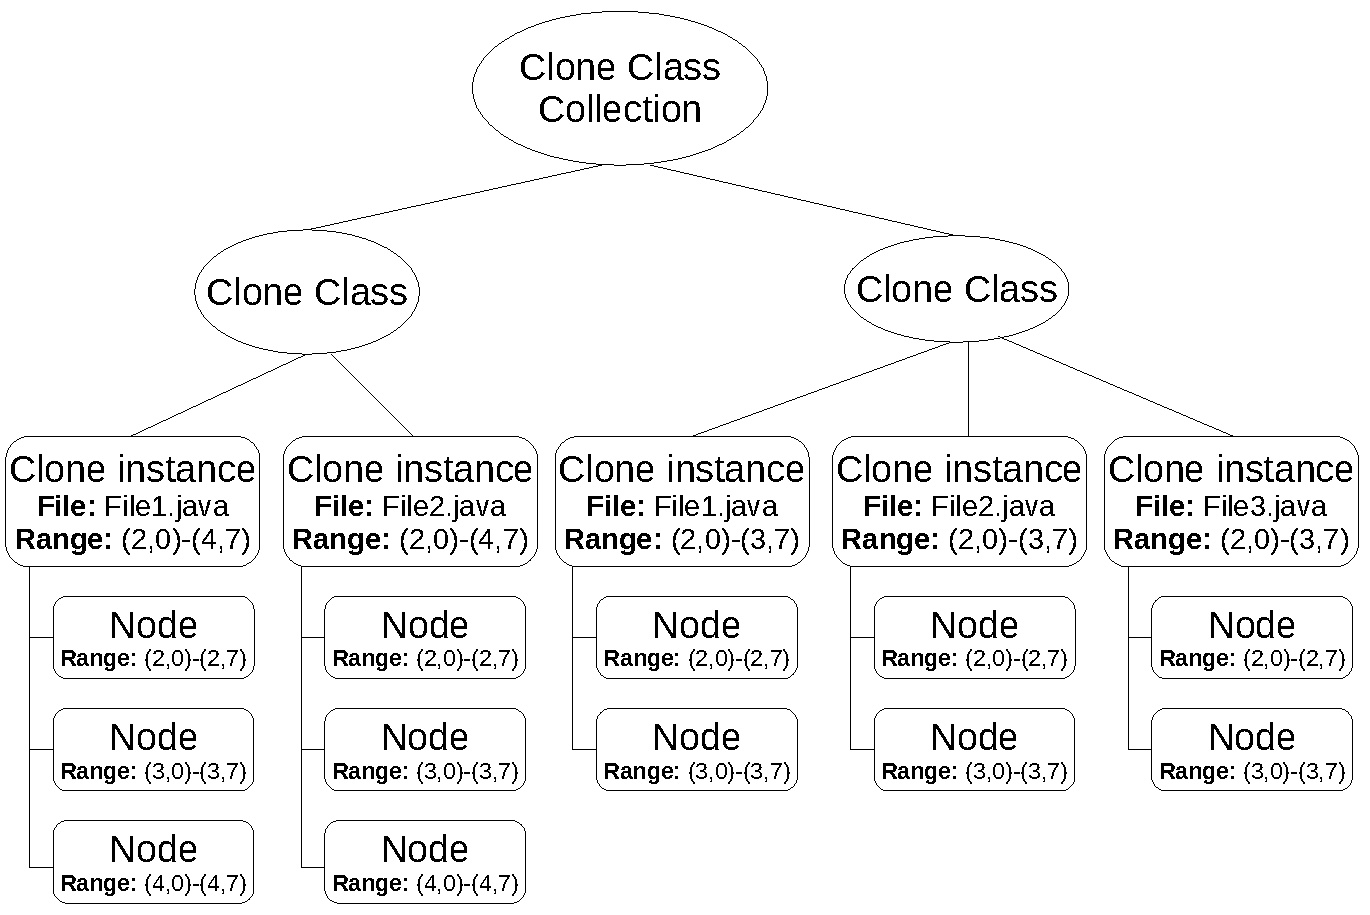
\includegraphics[width=1\columnwidth]{img/TerminologyExample}
  \caption{Representation of figure \ref{fig:cloneclasses} using the terminology introduced in table \ref{tab:clone-terminology}}
  \label{fig:terminologyexample}
\end{figure}

\section{Clone Types} \label{chap:backgroundclonetypes}
Duplication in code is found in many different forms. Most often duplicated code is the result of a programmer reusing previously written code \cite{haefliger2008code, baxter1998clone}. Sometimes this code is then adapted to fit the new context. To reason about these modifications, several clone types have been proposed. These clone types are described in Roy et al \cite{roy2007survey}:
\begin{displayquote}
\textbf{Type I:} Identical code fragments except for variations in whitespace (may be also variations in layout) and comments.\\
\textbf{Type II:} Structurally/syntactically identical fragments except for variations in identifiers, literals, types, layout and comments.\\
\textbf{Type III:} Copied fragments with further modifications. Statements can be changed, added or removed in addition to variations in identifiers, literals, types, layout and comments.\\
\textbf{Type IV:} Two or more code fragments that perform the same computation but implemented through different syntactic variants.
\end{displayquote}
A higher type of clone means that it's harder to detect and refactor. There are many studies that adopt these clone types, analyzing them further and writing detection techniques for them \cite{sajnani2016sourcerercc, kodhai2010detection, van2019novel}.

\subsection{Type 4 clones}
For this study we have chosen to take type 4 clones out of the scope, because they are both hard to detect and hard to refactor. A study by Kodhai et al \cite{kodhai2013method} looks into the distribution of the different types of clones in several open source systems (see table 6 of his study). It becomes apparent that type 4 clones exist way less in source code than all of the other types of clones. For instance, for the J2sdk-swing system he finds 8115 type 1 clones, 8205 type 2 clones, 11209 type 3 clones and only 30 type 4 clones. Because of that, we can conclude that type 4 clones are relatively less relevant to study.

\section{Refactoring methods}
One of the main drivers for starting this research is the recent release of the second edition of Martin Fowlers' Refactoring book \ref{fowler2018refactoring}. This book has been updated to the modern state of software engineering. The sentence in which he stresses the importance of unifying duplication in source code remains present in both books \ref{fowler1999refactoring, fowler2018refactoring}.

The main method for dealing with duplication in source code, as described by Martin Fowler, is to extract the duplication to a common place. In most IDE's this refactoring method is called ``Extract Method''.

\subsection{Extract Method}
Method extraction is one of the most used methods of refactoring duplication in source code. Several studies have already concluded that most duplication in source code is found in the body of methods \ref{lozano2007evaluating, white2016deep, bergman2004ethnographic}. Method extraction can move matching functionality between methods to a common place: a new method. An example of this procedure is displayed in figure \ref{fig:extractmethod}.

\begin{figure}[H]
\begin{parcolumns}{2}
\colchunk[1]{
\begin{javacode}
// Original
public void doStuff(){
|\highlightYellow|  doA();
|\highlightYellow|  doB();
  doC();
|\highlightYellow|  doA();
|\highlightYellow|  doB();
}
\end{javacode}}
\colchunk[2]{
\begin{javacode}
// Refactored
public void doStuff(){
|\highlightYellow|  doAandB();
  doC();
|\highlightYellow|  doAandB();
}

public void doAandB(){
  doA();
  doB();
}
\end{javacode}}
\end{parcolumns}
\caption{Refactoring duplication through method extraction.}
\label{fig:extractmethod}
\end{figure}

\subsection{Move method}
In the example of the previous section, both duplicated parts are in the same method. However, a study by Fontana et al. \ref{fontana2015duplicated} shows that this is most often not the case. Based on the relation between clone instances, the extracted method must be moved to be accessible by all locations of the clone instances. This might require different techniques.

\subsubsection{Pull up method}
A refactoring technique to move a method up in its inheritance structure is called ``Pull up method'' \ref{fowler2018refactoring}. This way, if cloned methods are related in any way through inheritance, they can be called by both classes by placing the method in a class they both have in common. This way its possible to refactor both fully cloned methods (by just pulling up the method) and partially cloned methods (by first performing method extraction and then pulling up the refactored method).

\subsubsection{Create class abstraction based on implicit relations}
Duplication in source code is an implicit relation between fragments of source code. If two classes have many of these implicit relations, then the implementation should be refactored to make this relation explicit. If the classes do not yet have a parent/super class, a parent class can be created and the common functionality can be placed in this newly created class. This makes the relation between these classes explicit and reduces duplication.

\subsubsection{Providing default implementations for common functionality}
Looking specifically at the Java programming language, recent versions of Java introduce a new method of reducing duplication through refactoring. Java has the concept of \textit{interfaces} as an abstract type that is used to specify a behavior that classes must implement. Since Java version 8, Java also supports default implementations to be provided in interfaces. This gives an opportunity to make the relation between classes explicit and reduce duplication. It can be used in instances where creating a new parent class for duplicated classes is undesirable.

\section{Clone Contexts} %I don't really like this chapter.
Code clones can be found anywhere in the code. The most commonly studied type of clone is the method-level clone. Method-level clones are duplicated blocks of code in the body of a method. Many clone detection tools only focus on method-level clones (like CPD\footnote{CPD is part of PMD, a commonly used source code analyzer: \url{https://github.com/pmd/pmd}}, Siamese\footnote{Siamese is an Elasticsearch based clone detector: \url{https://github.com/UCL-CREST/Siamese}}, Sysiphus\footnote{Sisyphus crawls the Java library for existing implementations of parts of a codebase: \url{https://github.com/fruffy/Sisyphus}}). The reason for this is that with method-level clones it's most likely that the clones are harmful, and they are more straight-forward to refactor.

A paper by Lozano et al \cite{lozano2007evaluating} discusses the harmfulness of cloning. In this paper the author argues that 98\% are produced at method-level. However, the paper that is cited to support this claim \cite{bergman2004ethnographic} does not conclude this same information. First of all, the study that is referenced uses a very small dataset (460 copy \& paste instances by 11 participants). Secondly, the group of subject only consists of IBM researchers (selection bias). Thirdly, it only focuses on copy and paste instances, as opposed to other ways clones can creep into the code. Finally, the ``98\%'' is not stated explicitly, but is vaguely derivable from one of the figures (figure 1) in this paper. Because of this, there is no reliable overview of how many clones there are in different contexts.

This thesis will focus on measuring how many clones there are per context. This way we can determine the impact of focusing our search on a specific context, like the analysis of only method-level clones. Our hypothesis is that the 98\% claim is not true (we think this should be far less). We also hypothesize that clones in different contexts than method-level are less likely to be harmful and less straight forward to refactor.

\subsection{Clone refactoring in relationship to its context}
How to refactor clones is highly dependent on their context. Method-level clones can be extracted to a method \cite{kodhai2013method} if all occurrences of the clone reside in the same class. If a method level clone is duplicated among classes in the same inheritance structure, we might need to pull-up a method in the inheritance structure. If instances of a method level clone are not in the same inheritance structure, we might need to either make a static method or create an inheritance structure ourselves. So not only a single instance of a clone has a context, but also the relationship between individual instances in a clone class. This is highly relevant to the way in which the clone has to be refactored.

\section{Code clone harmfulness}
There has been a lot of discussion whether code clones should be considered harmful.

Most papers view clones as harmful regarding program maintainability. \textit{``Clones are problematic for the maintainability of a program, because if the clone is altered at one location to correct an erroneous behaviour, you cannot be sure that this correction is applied to all the cloned code as well. Additionally, the code base size increases unnecessarily and so increases the amount of code to be handled when conducting maintenance work.''} \cite{ostberg2014automatically}

However, the harmfulness of clones depends on a lot of factors. A paper by Kapser et al \cite{kapser2006cloning} describes several patterns of cloning that may not be considered harmful. In this paper Kapser names examples where eliminating clones would compromise other important program qualities. Another study by Jarzabek et al \cite{jarzabek2010clones} categorized ``Essential clones'': clones that are essential because of the solution that is being modelled by the program. Overall, many of the benefits of code clones do not apply to most modern object-oriented programming languages.
